%\documentclass[12pt]{article}
%\usepackage[a4paper, margin=1in]{geometry} 
%\usepackage{graphicx} 
%\usepackage{hyperref}
%\usepackage{float}
%\usepackage{multicol}
%\usepackage{multirow}
%\usepackage[font=small, labelfont=bf]{caption}
%
%\begin{document}

%
% Evaluation of binary classifiers 
%
\subsection{Evaluation of binary classifiers}
Binary classifiers are mathematical or computational models that classify an input data set and produce the output with two labels. 

%
% Evaluation of models
%
\subsubsection*{Evaluation of models}
The performance of different models can be evaluated under the same test dataset.
\begin{itemize}
\item Algorithms
\item Scoring schemes
\item Statistical analysis
\end{itemize}

%
% Test data
%
\subsubsection*{Test data}
It should contain both homologous and non-homologous alignments.
\begin{itemize}
\item Positive: homologous
\item Negative: non-homologous
\end{itemize}

\begin{figure}[H]
  \centering
      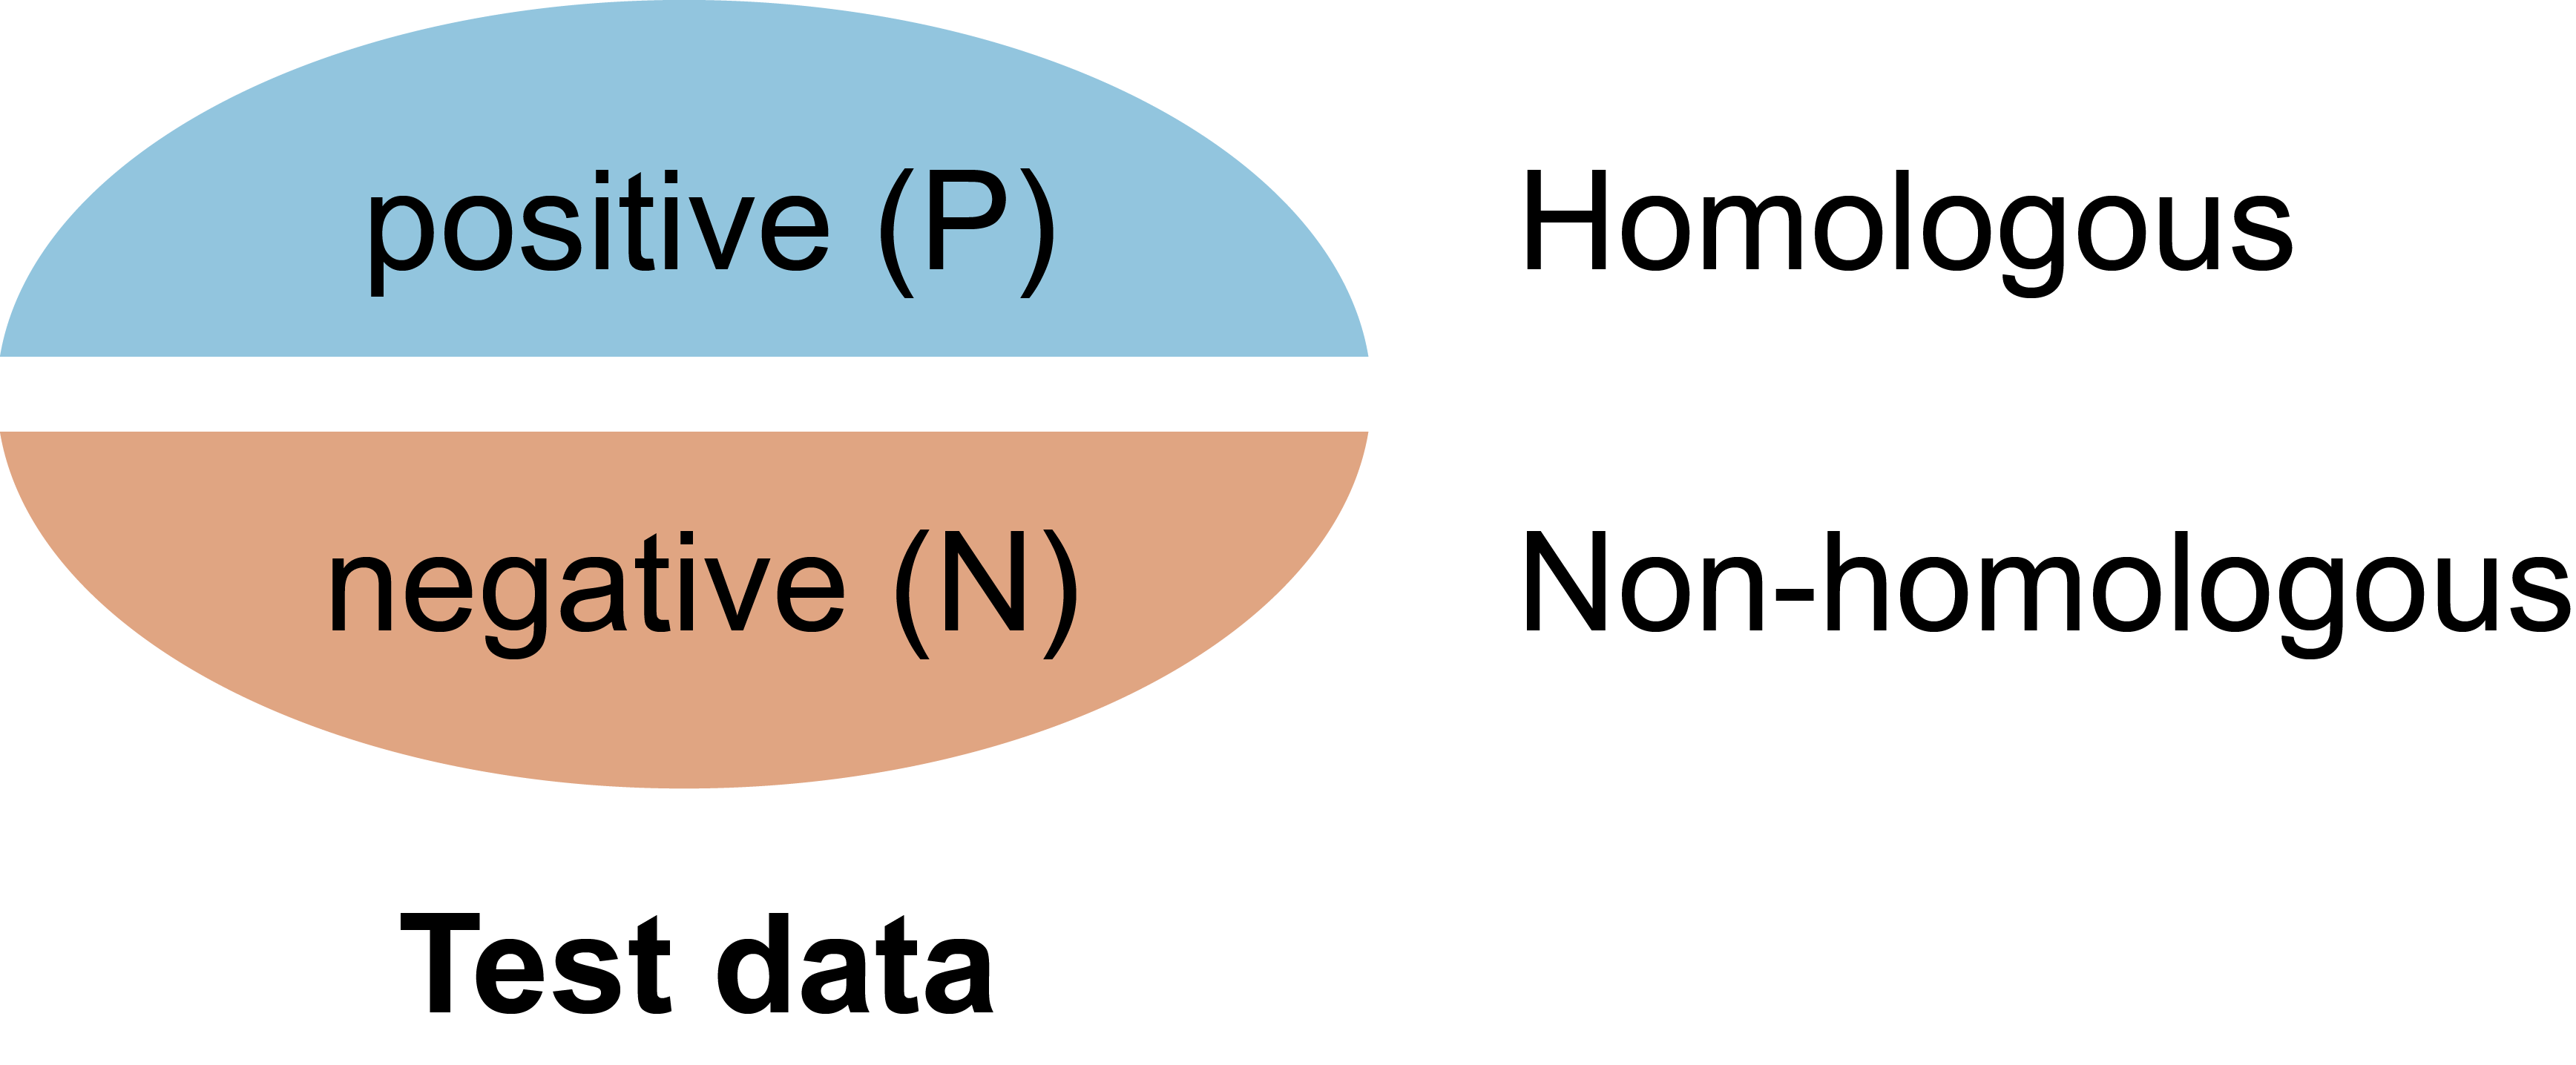
\includegraphics[width=0.4 \textwidth]{fig07/test_data.png}
  \caption{Test dataset for homologous and non-homologous}
\end{figure}

%
% Model output
%
\subsubsection*{Model output} 
Different models often output different formats of scores. 

\begin{itemize}
\item Raw scores, bit scores, z-scores
\item P-values, e-values
\end{itemize}

\noindent
Threshold values are used to separate the result into positives and negatives.

\begin{figure}[H]
  \centering
      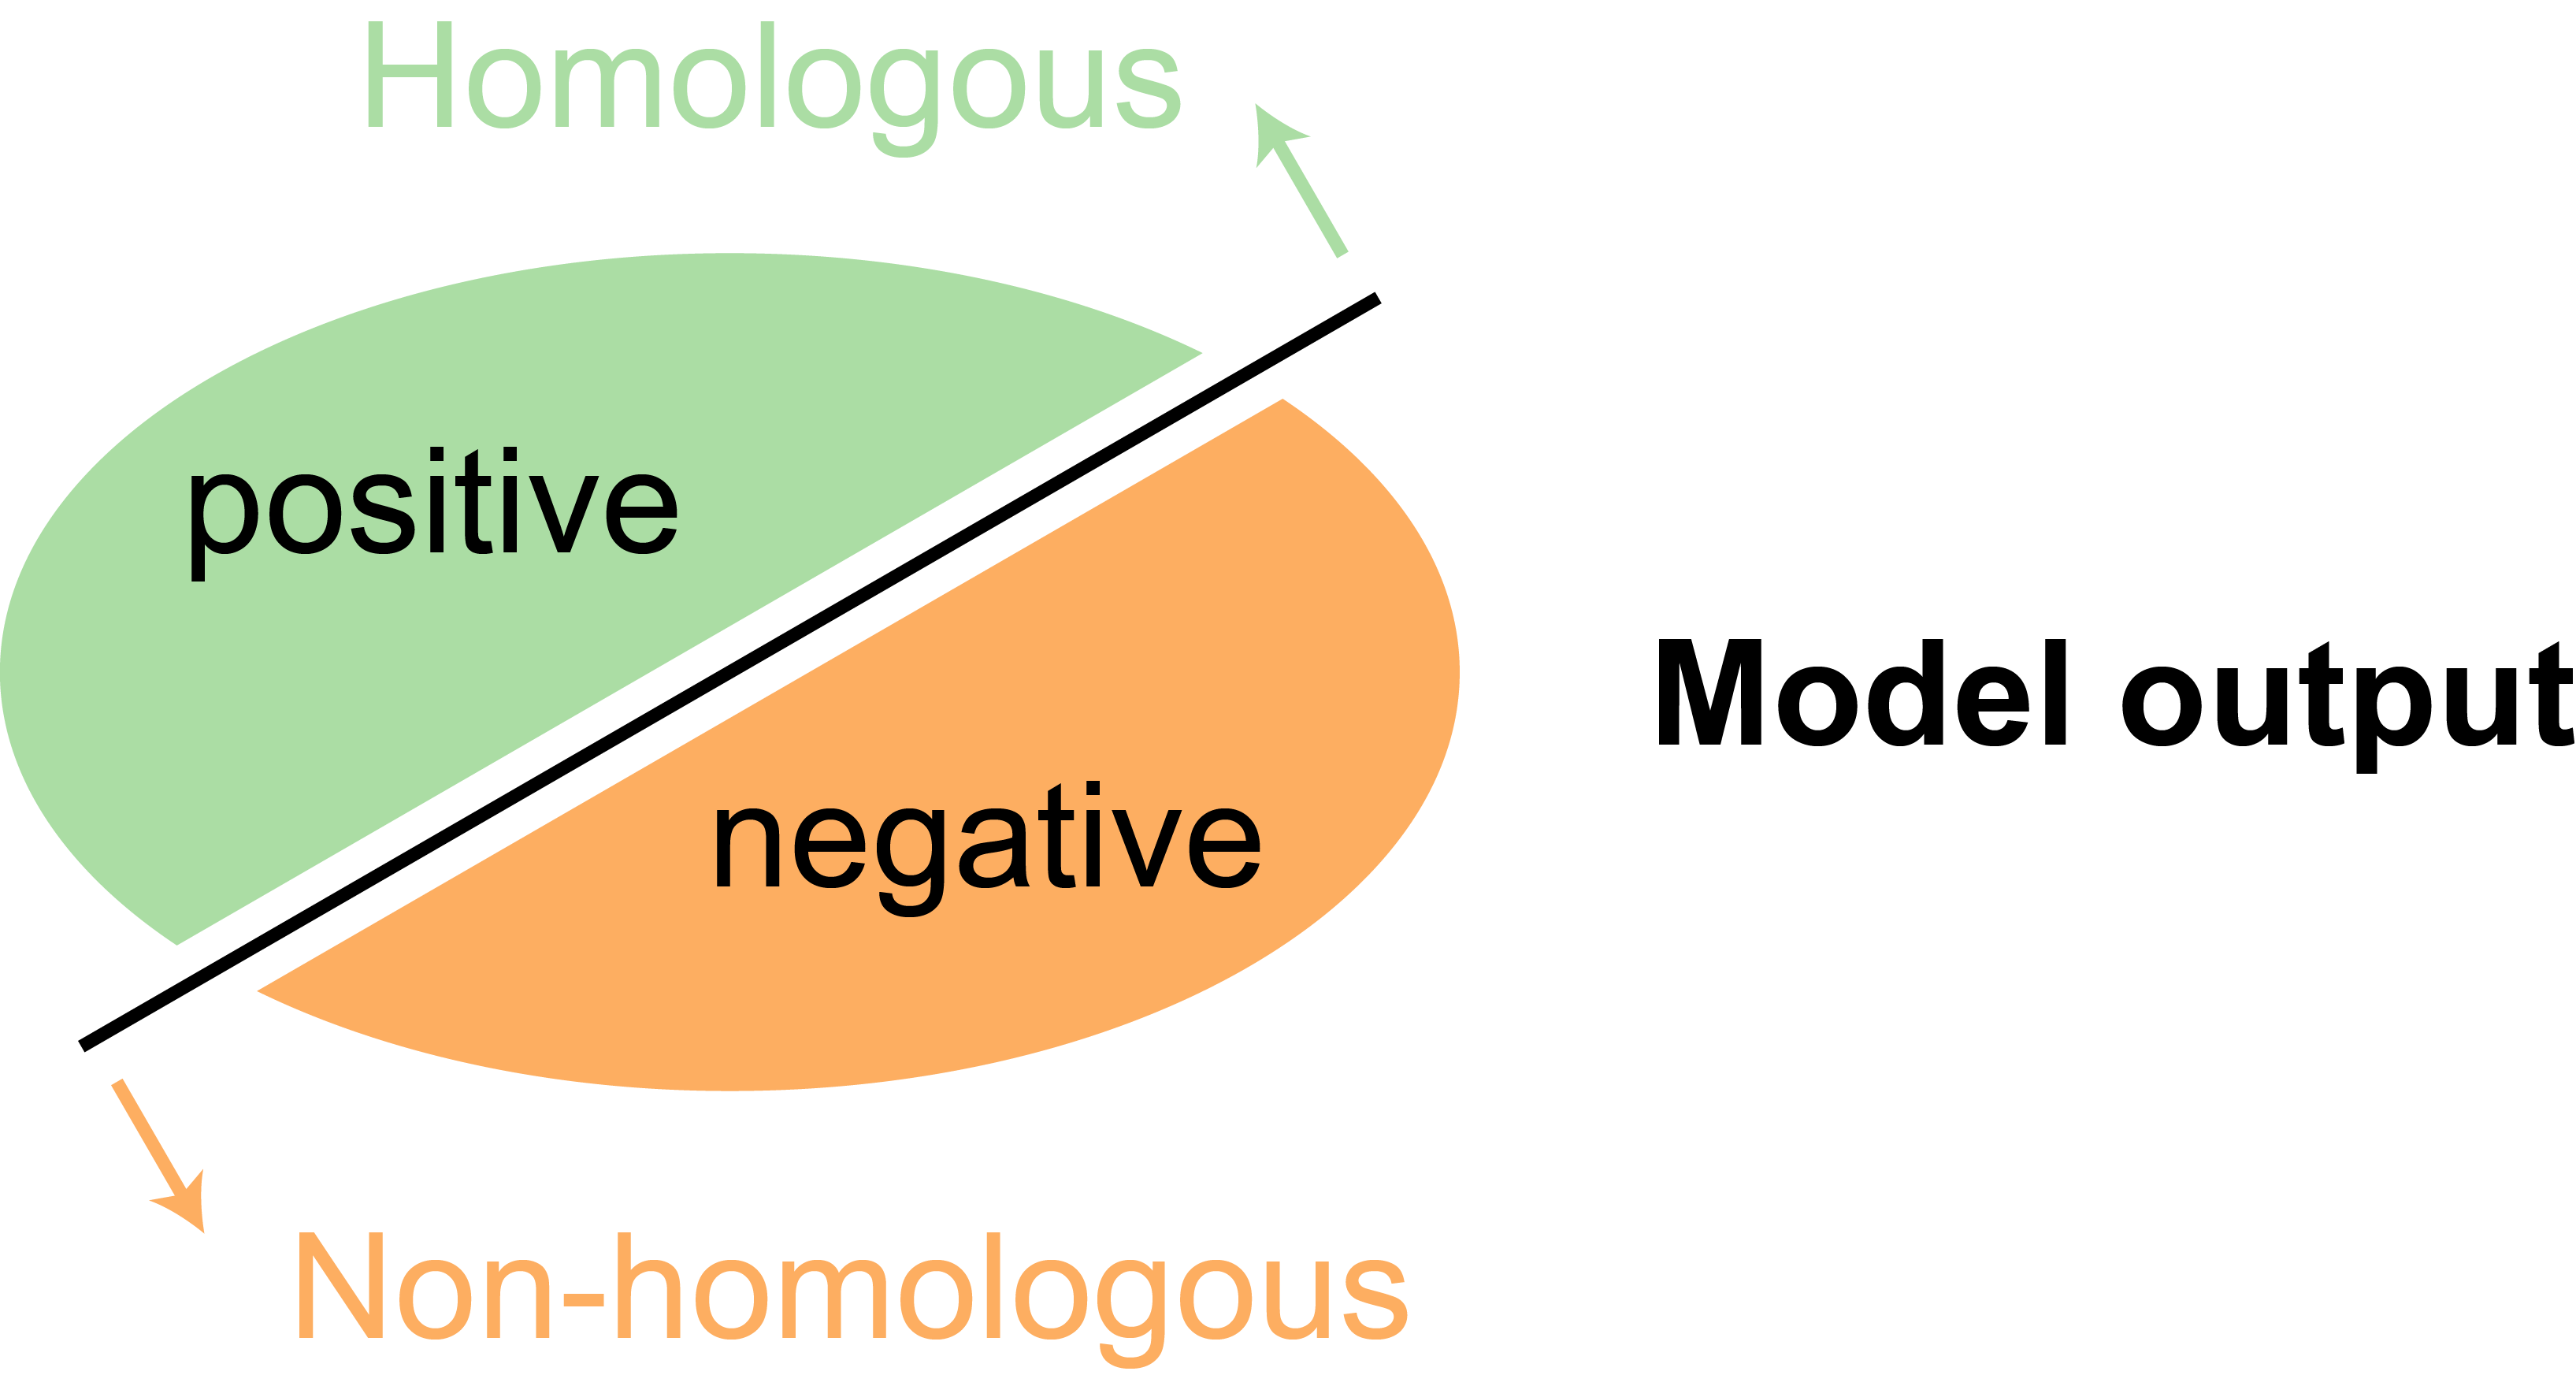
\includegraphics[width=0.4 \textwidth]{fig07/model_output.png}
  \caption{Model output for homologous and non-homologous}
\end{figure}

\bigskip 

%\end{document}
